\documentclass[conference]{IEEEtran}
\IEEEoverridecommandlockouts
% The preceding line is only needed to identify funding in the first footnote. If that is unneeded, please comment it out.
\usepackage{cite}
\usepackage{amsmath,amssymb,amsfonts}
\usepackage{algorithmic}
\usepackage{graphicx}
\usepackage{textcomp}
\usepackage{xcolor}
\usepackage{moreverb}
\usepackage{hyperref}
\def\BibTeX{{\rm B\kern-.05em{\sc i\kern-.025em b}\kern-.08em
    T\kern-.1667em\lower.7ex\hbox{E}\kern-.125emX}}
\begin{document}

\title{Text Classification Competition: Twitter Sarcasm Detection}

\author{
	\IEEEauthorblockN{Artsiom Strok}
	\IEEEauthorblockA{\textit{astrok2@illinois.edu}}
\and
	\IEEEauthorblockN{Peter Zukerman}
	\IEEEauthorblockA{\textit{peterz2@illinois.edu}}
\and
	\IEEEauthorblockN{Dheeraj Patta}
	\IEEEauthorblockA{\textit{npatta2@illinois.edu}}
	}

\maketitle

\begin{abstract}
We are exploring different machine learning models and NLP techniques to classify tweets as sarcastic or not. We tried classical algorithms such as Naive Bayes, Gradient Boosting, SVM, Random Forest, and deep learning algorithms such as LSTM, CNN, using various word embeddings. And finally, we used the BERT-large model to achieve the best results. We also explored different text pre-processing techniques, experimented with the context of the tweets, and tried to use additional information such as the tweet's sentiment.
\end{abstract}

\begin{IEEEkeywords}
Sarcasm, NLP, Figurative Language, Deep Learning, BERT, CNN, LSTM, Word2Vec.
\end{IEEEkeywords}

\section{Introduction}

Due to the growing volume of available textual information, there is a great demand for Natural Language Processing (NLP) techniques that can automatically process and manage texts, supporting the information retrieval and communication in core areas of society (e.g. healthcare, business, and science). NLP techniques have to tackle the often ambiguous and linguistic structures that people use in everyday speech. As such, there are many issues that have to be considered, for instance slang, grammatical errors, regional dialects, figurative language, etc. Figurative Language (FL), such as irony, sarcasm, similes, and metaphors, pose a serious challenge to NLP systems. FL is a frequent phenomenon within human communication, occurring both in spoken and written discourse including books, websites, forums, chats, social network posts, news articles and product reviews. \cite{b1}

\section{Data}

\subsection{Dataset format}

Each line contains a JSON object with the following fields:

\begin{itemize}
	\item\textbf{\emph{response}} : the Tweet to be classified
	\item\textbf{\emph{context}} : the conversation context of the
	\item\textbf{\emph{response}} - Note, the context is an ordered list of dialogue, i.e., if the context contains three elements, \texttt{c1}, \texttt{c2}, \texttt{c3}, in that order, then \texttt{c2} is a reply to \texttt{c1} and \texttt{c3} is a reply to \texttt{c2}. Further, the Tweet to be classified is a reply to \texttt{c3}.
	\item\textbf{\emph{label}} : \texttt{SARCASM} or \texttt{NOT\_SARCASM}
\end{itemize}

\subsection{Example}

\begin{verbatimtab}[4]
"label": "SARCASM", 
"response": 
	"@USER @USER @USER I don't 
	get this .. obviously you do care
	or you would've moved right along ..
	instead you decided to care and
	troll her ..",
 "context": 
 	"A minor child deserves privacy and
	should be kept out of politics.
	Pamela Karlan, you should be ashamed
	of your very angry and obviously
	biased public pandering, and using a child
	to do it .",
	
	"@USER If your child isn't named Barron ...
	\#BeBest Melania couldn't care less. Fact "
	
\end{verbatimtab}


The response tweet, 
\begin{verbatim}
@USER @USER @USER I don't get this ...
\end{verbatim}
is a reply to its immediate context
\begin{verbatim}
@USER If your child isn't ...
\end{verbatim}
which is a reply to
\begin{verbatim}
A minor child deserves privacy ...
\end{verbatim}


\begin{table}[htbp]
\caption{Dataset size statistics}
\begin{center}
\begin{tabular}{|l|l|}
\hline
\textbf{Train} & \textbf{Test} \\ \hline
5000 & 1800          \\ \hline
\end{tabular}
\label{tab1}
\end{center}
\end{table}

\section{Experiments}
The source code of all experiments is available on \href{https://github.com/dheerajpatta/CourseProject}{GitHub}.

\subsection{Project plan}

Our team had clarity on the roles/responsibilities and categorized the task of classifying twitter sarcasm detection as follows:

\begin{itemize}
	\item Understanding Data
	\item Data enrichment and pre-processing
	\item Implementing classic algorithms
	\item Research on SoTA models and Glue Leaderboard\footnote{https://super.gluebenchmark.com/leaderboard/}
	\item Implementing State-of-the-Art Models
	\item Evaluation and Fine-tuning
	\item Current Leaderboard
\end{itemize}

\subsection{Data enrichment and pre-processing}
We’ve performed comprehensive Exploratory Data Analysis (EDA) on the given training dataset using traditional methods as well as the dedicated pre-processing python package ``ekphrasis`` to understand the dataset attributes like distribution, tokenization, lemmatization, normalization, annotation, spell correction, label encoding and word segmentation. This enriched training data is then used to train classic and SoTA models to predict the sarcasm responses. 
\subsection{Initial Modeling and Thoughts}
The language of our choice is Python, and we started with simple yet powerful framework/library ``sklearn`` to implement classic models like Naïve Bayes (Multinomial), linear models like SGD (Stochastic Gradient Descent) and ensembles like Gradient Boosting.
We’ve utilized stratified ``k-folds`` cross validation and split the dataset into 5 folds for cross training and validation. 
\begin{verbatimtab}[4]
skf = StratifiedKFold(
	n_splits=5,
	random_state=123,
	shuffle=True)
\end{verbatimtab}
The initial round of classical methods used are Count Vectorizer, TF-IDF transformer and Multinomial Naïve Bayes.
\begin{verbatimtab}[4]
text_clf = Pipeline([
    ('vect', CountVectorizer()),
    ('tfidf', TfidfTransformer()),
    ('clf', MultinomialNB()),
])
\end{verbatimtab}
Using Macro average precision, here are the results for our initial round of modeling.
We’ve introduced tokenization and word lemmatization to study the effect of the same on dataset and with ensemble methods like boosting. (XGB and GB)
\begin{verbatimtab}[4]
Pipeline([
    ('vect', CountVectorizer(
    	strip_accents = 'unicode',
         stop_words = 'english',
         lowercase = True)),
    ('tfidf', TfidfTransformer()),
    ('clf', GradientBoostingClassifier()),
])
\end{verbatimtab}
\begin{table}[htbp]
	\caption{Classical ML algorithms performance}
	\begin{center}
		\begin{tabular}{|l|l|l|l|}
			\hline
			\textbf{Model} & \textbf{Precision} & \textbf{Recall} & \textbf{F1}\\ \hline
			Multinomial Naïve Bayes & 0.7349 & 0.7808 & 0.7570 \\ \hline
			XGBoost & 0.6548 & 0.7744 & 0.7095 \\ \hline
		\end{tabular}
		\label{tab2}
	\end{center}
\end{table}
\begin{table}[htbp]
	\caption{Auto Scikit Learn results}
	\begin{center}
		\begin{tabular}{|l|l|}
			\hline
			\textbf{Model} & \textbf{Accuracy}\\ \hline
			LibSVM (SVC) & 0.7770 \\ \hline
			Random Forest & 0.7624 \\ \hline
			Bernoulli NB & 0.7545 \\ \hline
			SGD & 0.7509 \\ \hline
			Extra Trees & 0.7491 \\ \hline
			Passive Aggressive & 0.7412 \\ \hline
			LibLinear (SVC) & 0.7388 \\ \hline
			AdaBoost & 0.7176 \\ \hline
			KNN & 0.6921 \\ \hline
			DT & 0.6321 \\ \hline								
		\end{tabular}
		\label{tab2}
	\end{center}
\end{table}
Although the results are encouraging, we couldn’t surpass the baseline.
\subsection{Deep Neural Network (CNN, LSTM)}
We’ve progressed to build a Deep Learning model and based on our study on research papers published in the domain of sentiment analysis and sarcasm analysis, we’ve chosen to use Convolution Neural Networks and Long Short-Term Memory (LSTM) deep learning techniques to classify the twitter sarcasm dataset.
The framework of our choice is TensorFlow with Keras (a high-level abstraction layer) for building a Deep Learning model. We’ve followed a well established and documented process of DL model building using Keras. Below is the summary of our DL Model including Hidden layers.
\begin{figure}[htbp]
\centerline{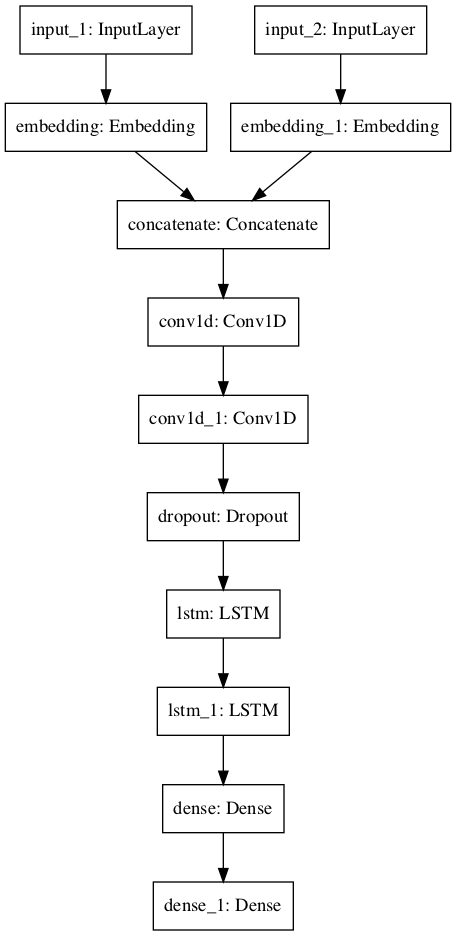
\includegraphics[width=0.6\columnwidth]{model.PNG}}
\caption{Deep Learning model architechture}
\label{fig1}
\end{figure}
\begin{figure}[htbp]
\centerline{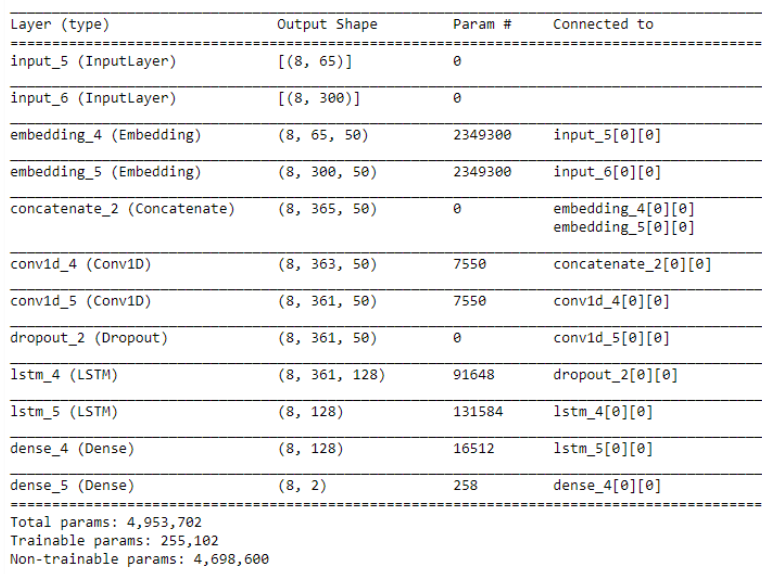
\includegraphics[width=1\columnwidth]{poorModel.PNG}}
\caption{Layer Dimensions}
\label{fig2}
\end{figure}



However, the model did not perform well, likely due to the lack of data and performed poorly than classic models (our first iteration)
\subsection{State-Of-The-Art (SoTA) Models}
The GLUE benchmark leaderboard in NLP is dominated by BERT and incremental updates/flavors of BERT. This is an incredible opportunity for us to implement some of the state-of-the-art models. 
We’ve utilized Google Colab to make use of in-built NVIDIA GPUs and computational power to train our BERT model.
The model is trained on GPUs for 15 epochs with a batch size of 24. We’ve saved the model weights, parameters and checkpoints to a hdf5 file format (as recommended by TensorFlow). The weights are then loaded to perform predictions and are saved to answer.txt.
This is clearly a Winner. We’ve successfully beat the baseline and achieved a ranking of \#2 in leaderboard.
\begin{figure}[htbp]
\centerline{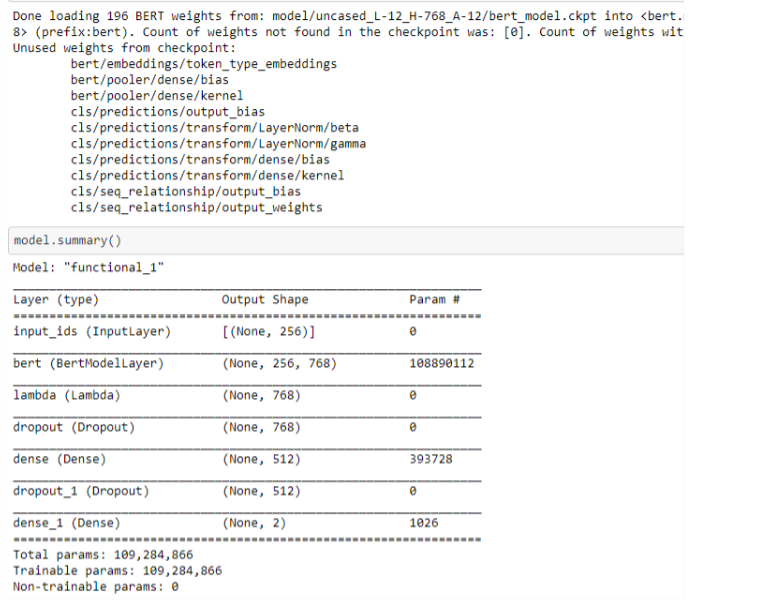
\includegraphics[width=1\columnwidth]{bert.PNG}}
\caption{BERT - Layer Dimensions}
\label{fig3}
\end{figure}

\section{Results}
\subsection{Closing thoughts}
We are working towards fine-tuning the winning model by augmenting "rich" data like sentiments, emoticons understanding, context and relationships. We are currently focusing on implementing the different flavors of BERT like Facebook’s RoBERTa, ALBERT with NAS, ERNIE and Google T5 to see if there is any significant improvement in our prediction accuracy and F1 scores thereby pushing our team to \#1 in the Leaderboard.

\begin{thebibliography}{00}
	\bibitem{b1} Weitzel, Leila \& Prati, Ronaldo \& Aguiar, Raul. (2016). ``The Comprehension of Figurative Language: What Is the Influence of Irony and Sarcasm on NLP Techniques?`` 10.1007/978-3-319-30319-2\_3. 
	\bibitem{b2} Lee, H., Yu, Y., and Kim, G., “Augmenting Data for Sarcasm Detection with Unlabeled Conversation Context”, \textit{arXiv e-prints}, 2020.
	\bibitem{b3} Dong, X., Li, C., and Choi, J. D., “Transformer-based Context-aware Sarcasm Detection in Conversation Threads from Social Media”, \textit{arXiv e-prints}, 2020.
	\bibitem{b4} Pant, K. and Dadu, T., “Sarcasm Detection using Context Separators in Online Discourse”, \textit{arXiv e-prints}, 2020.
	\bibitem{b5} González-Ibáñez, R.I., Muresan, S., \& Wacholder, N. (2011). Identifying Sarcasm in Twitter: A Closer Look. ACL.
	\bibitem{b6} SoTA Sarcasm Detection Benchmarks \url{https://paperswithcode.com/task/sarcasm-detection/codeless}
\end{thebibliography}
\appendices
\section{Submission history}
\begin{table}[htbp]
	\caption{Submission history}
	\begin{center}
		\begin{tabular}{|l|l|l|l|l|l|}
			\hline
			\textbf{Model} & \textbf{Precision} & \textbf{Recall} & \textbf{F1} & \textbf{Beat the baseline} & \textbf{Rank} \\ \hline
			Classic & 0.681 & 0.684 & 0.683 & No  & 34 \\ \hline
			BERT & 0.691 & 0.845 & 0.761 & Yes  & 2 \\ \hline
			BERT+Sentiment & 0.692 & 0.845 & 0.761 & Yes & 5 \\ \hline
		\end{tabular}
		\label{tab3}
	\end{center}
\end{table}
\end{document}